% College Lecture 14: message integrity, birthday problems, hash attacks, iterated hashes, SHA-512, Whirlpool.
% Sources: slides L14 (58 slides), Forouzan ch. 11 + 12. Every number recomputed by script (scratchpad/hash/verify*.py).
\section{Message Integrity and Hash Functions}\label{sec:integrity}
\usetikzlibrary{decorations.pathreplacing}

\subsection{Integrity versus secrecy; message and digest \new}
\likely{``Why is a hash, not encryption, used for integrity?'' and ``how is integrity checked with a digest?'' (2--3 marks).}

Every scheme so far gave \emph{secrecy}: Eve cannot read the message. Many documents need the opposite guarantee. Alice's will, for example, need not be encrypted, because after her death anyone may read it; what must be preserved is its \emph{integrity}, meaning that nobody can change its contents without the change being noticed. On paper this is achieved by putting Alice's fingerprint at the bottom of the document: Eve can read the will, but she cannot alter it or write a false one, because she cannot forge the fingerprint.

The electronic equivalent of the document--fingerprint pair is the \textbf{message--digest pair}. The message is passed through a \textbf{cryptographic hash function} $h$, which maps a message of any length to a short fixed-length string $h(M)$, called the \textbf{message digest}. The digest is a compressed image of the message that plays the role of the fingerprint. To check integrity later, the receiver runs the same hash function on the message he now holds and compares the new digest with the stored one: \imp{if the two digests are equal, the message has not been changed; if they differ, the message was changed and is discarded.}

\textbf{Why a hash and not encryption.} Encryption hides the message but does not stop Eve from altering the ciphertext; flipping a bit of a one-time-pad or stream-cipher ciphertext flips the same bit of the plaintext, and Bob has no way to tell a changed plaintext from a genuine one. A hash works the other way round: it hides nothing (the message can be public), but since any change to the message produces a different digest, any change is detected. The two services are therefore independent, and a message can need one, the other, or both.

\textbf{The digest itself must be safe.} The check only works if the stored or received digest is genuine. If Eve can replace both $M$ and $h(M)$, she simply sends $M'$ with $h(M')$ and the comparison passes. Hence the digest is kept in a safe place or sent over an authenticated channel; binding the digest to a secret key gives the MAC of the next lecture.

\subsection{The three security criteria \new}
\likely{``Define and differentiate preimage, second preimage and collision resistance'' (3--4 marks), possibly with a figure of what Eve is given and must find.}

A cryptographic hash function must make three kinds of forgery infeasible. They differ in how much Eve is given at the start, and therefore in how much freedom she has.

\textbf{Preimage resistance.} Given a hash function $h$ and a digest $y = h(M)$, it must be extremely difficult for Eve to find \emph{any} message $M'$ with $h(M') = y$. If $h$ were not preimage resistant, Eve could intercept just the digest $h(M)$, construct a message $M'$ that hashes to it, and send $M'$ to Bob as if it were $M$. In other words, the hash must be one-way.

\textbf{Second preimage resistance.} Given a specific message $M$ \emph{and} its digest $h(M)$, it must be extremely difficult to find another message $M' \ne M$ with $h(M') = h(M)$. This is the criterion that stops forgery of a particular message: if Alice sends $M$ and $h(M)$ to Bob, Eve cannot create a different message with the same digest and substitute it. Eve here has more information than in the preimage case (she also knows one valid preimage), but she still has to hit one fixed target value.

\textbf{Collision resistance.} It must be extremely difficult to find \emph{any} two messages $M \ne M'$ with $h(M) = h(M')$. Here Eve is given nothing and is free to choose both messages from scratch; such a pair is called a \textbf{collision}. This is the danger when Eve prepares two documents herself (say a fair contract and an unfair one with the same digest), gets Alice to approve the fair one, and later swaps in the other.

\begin{center}\small
\begin{tabularx}{\textwidth}{@{}l X X l@{}}
\toprule
Criterion & Eve is given & Eve must find & Attack it stops\\
\midrule
Preimage resistance & $h$ and a digest $y = h(M)$ & any $M'$ with $h(M') = y$ & preimage\\
Second preimage resistance & $h$, a message $M$ and $h(M)$ & $M' \ne M$ with $h(M') = h(M)$ & second preimage\\
Collision resistance & only $h$ & any pair $M \ne M'$ with $h(M) = h(M')$ & collision\\
\bottomrule
\end{tabularx}
\end{center}

\textbf{Collision resistance implies second preimage resistance.} Suppose Eve had a method that, given any $M$, produces a second preimage $M'$. She could then pick any $M$ she likes, run the method, and output the pair $(M, M')$, which is a collision. So a function that is \emph{not} second-preimage resistant cannot be collision resistant; equivalently, a collision-resistant function is automatically second-preimage resistant. The converse fails, because finding a collision is the easier task (Eve chooses both sides), and the birthday analysis below shows by how much: a collision costs about $2^{n/2}$ hash evaluations, a second preimage about $2^n$.

\textbf{Why a compressor or a checksum is not a cryptographic hash.} A lossless compression method such as ZIP or StuffIt also shrinks the message, but it is reversible: anyone can decompress the output and get the original, so it is not even a function to a fixed-length output, and it fails preimage resistance trivially. A checksum (adding up the bytes, a CRC) is fixed-length but linear and easy to invert: given a target checksum, Eve can compute what to change in any message to reach it, so it is neither preimage nor second-preimage resistant. Checksums detect accidental errors, not deliberate ones.

\begin{mustknow}[: the three criteria]
\textbf{Preimage}: given $y$, find any $M'$ with $h(M') = y$. \quad \textbf{Second preimage}: given $M$, find $M' \ne M$ with $h(M') = h(M)$. \quad \textbf{Collision}: find any $M \ne M'$ with $h(M) = h(M')$.\\
Cost for an ideal $n$-bit hash: preimage and second preimage $\approx 2^n$, collision $\approx 2^{n/2}$. Collision resistance $\Rightarrow$ second preimage resistance.
\end{mustknow}

\subsection{The random oracle model \new}
\likely{``Explain the random oracle model; why can the oracle not use a formula?'' (2--3 marks).}

To analyse attacks we need a model of a perfect hash function, against which real designs are compared. The \textbf{random oracle model} (Bellare and Rogaway, 1993) describes such an ideal function as an oracle that keeps a table of the messages it has already hashed and obeys three rules:
\begin{enumerate}[nosep]
  \item When a \emph{new} message of any length is given, the oracle creates a fixed-length digest that is a truly random string of 0s and 1s, gives it out, and records the message and digest in its table.
  \item When a message is given for which a digest already exists, the oracle simply returns the digest in the table. This makes the function deterministic: the same message always gets the same digest.
  \item The digest for a new message must be chosen independently of all previous digests. This implies that the oracle cannot use a formula or an algorithm to calculate the digest.
\end{enumerate}

\textbf{Example (slides 20--23).} An oracle with 16-bit digests already holds three entries. It is asked to hash \ttx{AB1234CD8765BDAD}, which is not in its table, so it flips a fair coin 16 times and gets \ttx{HHTHHHTTHTHHTTTH}. Reading H as 1 and T as 0 gives \ttx{1101 1100 1011 0001} $=$ \ttx{DCB1}, which it returns and records. When it is then asked for \ttx{4523AB1352CDEF45126}, which is already in the table, it does not flip again but returns the stored digest \ttx{13AB}.
\begin{center}\small
\begin{tabular}{@{}ll@{}}
\toprule
Message & Digest\\
\midrule
\ttx{4523AB1352CDEF45126} & \ttx{13AB}\\
\ttx{723BAE38F2AB3457AC} & \ttx{02CA}\\
\ttx{AB1234CD8765BDAD} & \ttx{DCB1} (new)\\
\ttx{AB45CD1048765412AAAB6662BE} & \ttx{A38B}\\
\bottomrule
\end{tabular}
\end{center}

\textbf{Why a formula violates rule 3.} Suppose the oracle used $h(M) = M \bmod n$ and had already issued $h(M_1)$ and $h(M_2)$. For the new message $M_3 = M_1 + M_2$ anyone can predict the digest without asking, since
\[
h(M_3) = (M_1 + M_2) \bmod n = [\,h(M_1) + h(M_2)\,] \bmod n .
\]
The digest of $M_3$ is therefore not independent of the earlier digests, which breaks rule 3. Real hash functions are algorithms, so they can only approximate the oracle; the model tells us the best security an $n$-bit design can hope for.

\textbf{What the model gives an attacker.} With an $n$-bit digest there are $N = 2^n$ possible digests, and each new message receives one of them uniformly at random. Some values may be chosen several times and some never. Eve knows the algorithm and $n$, so every attack reduces to drawing random digests and waiting for a match, which is exactly a birthday problem.

\subsection{The four birthday problems \new}
\likely{Derive the probability formula for one problem and get $k$ for $P = 1/2$; or ``how many people for a shared birthday'' (23).}

All four problems use a random variable that is uniform over $N$ values ($0$ to $N - 1$; $N = 365$ for birthdays) and ask for the minimum number of samples $k$ that makes an event \emph{likely}, meaning probability $P \ge 1/2$. Every derivation uses the approximation $1 - x \approx e^{-x}$ for small $x$.

\textbf{Problem 1: a sample equals a predefined value.} What is the minimum number of students such that it is likely that at least one has a \emph{predefined} birthday (say 1 January)? A single sample misses the target with probability $1 - 1/N$, and the $k$ samples are independent, so all of them miss with probability $(1 - 1/N)^k \approx e^{-k/N}$. Hence
\[
P_1 \approx 1 - e^{-k/N}, \qquad k \approx \ln\frac{1}{1-P}\times N \;\xrightarrow{P = 1/2}\; k \approx \ln 2 \times N = 0.69N .
\]
For $N = 365$: $0.693 \times 365 = 252.99$, so $k = 253$.

\textbf{Problem 2: a sample equals one chosen from the set.} What is the minimum number such that it is likely that at least one student has the same birthday as a student \emph{selected by the professor}? The selected student is one of the $k$, so only the other $k - 1$ can match, and the problem is Problem 1 with $k - 1$ samples:
\[
P_2 \approx 1 - e^{-(k-1)/N}, \qquad k \approx \ln 2 \times N + 1 = 0.69N + 1 ;\qquad N = 365:\ k = 254 .
\]

\textbf{Problem 3: any two samples are equal (the birthday paradox).} What is the minimum number such that it is likely that \emph{at least two} students share a birthday? It is easier to count the complement, that all $k$ values are different. The first value is free, the second must avoid 1 value, the $i$-th must avoid $i - 1$ values, so
\[
\Pr[\text{all different}] = \prod_{i=1}^{k-1}\Bigl(1 - \frac{i}{N}\Bigr) \approx \prod_{i=1}^{k-1} e^{-i/N} = e^{-(1 + 2 + \dots + (k-1))/N} = e^{-k(k-1)/2N}.
\]
Therefore
\[
P_3 \approx 1 - e^{-k(k-1)/2N}, \qquad k \approx \Bigl\{2\ln\frac{1}{1-P}\Bigr\}^{1/2} N^{1/2} \;\xrightarrow{P = 1/2}\; k \approx \sqrt{2\ln 2}\,\sqrt N = 1.18\sqrt N ,
\]
using $k(k-1) \approx k^2$. For $N = 365$: $1.18 \times 19.1 = 22.5$, so $k = 23$ (exactly, 23 people give $P = 0.507$ and 22 give $0.476$). The answer is a ``paradox'' only because intuition compares each person with \emph{one} date, whereas $k$ people form $k(k-1)/2 = 253$ pairs, each a chance to match.

\textbf{Problem 4: a sample of one set equals a sample of another.} Two classes each have $k$ students. What is the minimum $k$ such that it is likely that some student of the first class shares a birthday with some student of the second? Treat the $k$ values of set 1 as (nearly) distinct. Each value of set 2 then misses all of them with probability $1 - k/N$, and the $k$ values of set 2 all miss with probability $(1 - k/N)^k \approx e^{-k^2/N}$. Hence
\[
P_4 \approx 1 - e^{-k^2/N}, \qquad k \approx \Bigl\{\ln\frac{1}{1-P}\Bigr\}^{1/2} N^{1/2} \;\xrightarrow{P = 1/2}\; k \approx \sqrt{\ln 2}\,\sqrt N = 0.83\sqrt N ;\qquad N = 365:\ k = 16 .
\]
(Exactly, $k = 16$ gives $P = 0.504$.)

\begin{center}\small
\begin{tabular}{@{}clllcl@{}}
\toprule
Problem & Probability $P$ & General $k$ & $k$ at $P = \tfrac12$ & $N = 365$ & Attack\\
\midrule
1 & $1 - e^{-k/N}$ & $\ln\frac{1}{1-P} \cdot N$ & $0.69N$ & 253 & preimage\\
2 & $1 - e^{-(k-1)/N}$ & $\ln\frac{1}{1-P} \cdot N + 1$ & $0.69N + 1$ & 254 & second preimage\\
3 & $1 - e^{-k(k-1)/2N}$ & $\{2\ln\frac{1}{1-P}\}^{1/2} N^{1/2}$ & $1.18\sqrt N$ & 23 & collision\\
4 & $1 - e^{-k^2/N}$ & $\{\ln\frac{1}{1-P}\}^{1/2} N^{1/2}$ & $0.83\sqrt N$ & 16 & alternate collision\\
\bottomrule
\end{tabular}
\end{center}
The constants are $0.69 = \ln 2$, $1.18 = \sqrt{2\ln 2}$ and $0.83 = \sqrt{\ln 2}$. The key comparison is that \textbf{$k$ grows like $N$ in Problems 1 and 2 but only like $\sqrt N$ in Problems 3 and 4}. Problems 1 and 2 model the preimage and second preimage attacks, Problems 3 and 4 the collision attacks, so a collision attack is far cheaper than a preimage attack on the same hash.

\begin{trap}[: rounding the constant]
With $0.69$ exactly, $0.69 \times 365 = 251.85$, which would suggest 252; the table value 253 comes from $\ln 2 = 0.6931$ ($0.6931 \times 365 = 252.99$). Use $0.693$ when the answer must be an exact head count. Also do not mix up Problems 1 and 3: ``someone has \emph{my} birthday'' needs 253 people, ``\emph{some two} share a birthday'' needs only 23.
\end{trap}

\begin{worked}[: birthday numbers for a 16-bit digest]
\textbf{Q.} A hash function produces 16-bit digests. Using the birthday results, how many random messages must Eve hash for a probability of at least $1/2$ of (a) matching a given digest, (b) finding any two messages with the same digest, (c) a match between two lists of $k$ messages each?

\textbf{A.} $N = 2^{16} = 65\,536$ and $\sqrt N = 2^8 = 256$.\\
(a) Problem 1: $k \approx 0.69 \times 65\,536 \approx 45\,220$ messages (order $2^{16}$).\\
(b) Problem 3: $k \approx 1.18 \times 256 \approx \mathbf{302}$ messages (order $2^8$).\\
(c) Problem 4: $k \approx 0.83 \times 256 \approx \mathbf{213}$ messages in each list.\\
\emph{Check}: (b) is about 150 times cheaper than (a), as $2^{16}/2^8 = 256$ predicts up to the constants.
\end{worked}

\subsection{Attacks on an $n$-bit digest \new}
\likely{``A hash uses a 64-bit digest; how many digests must Eve create to find a collision (or the original message) with $P > 0.5$, and how long does it take?'' (3--4 marks).}

Assume the hash behaves like a random oracle with $n$-bit digests, so its outputs are uniform over $N = 2^n$ values, and that Eve knows the algorithm and $n$. Each attack below is a loop that creates messages, hashes them, and compares digests; its success probability is the matching birthday problem.

\textbf{Preimage attack.} Eve has intercepted a digest $D = h(M)$ and wants any $M'$ with $h(M') = D$. She creates $k$ messages $M[1], \dots, M[k]$, computes $T = h(M[i])$ for each, and returns $M[i]$ as soon as $T = D$. The target $D$ is a predefined value, so this is Problem 1: $P = 1 - e^{-k/N}$, and success with $P \ge 1/2$ needs $k = 0.69 \times 2^n$ digests, which is of order $2^n$.

\textbf{Second preimage attack.} Eve has intercepted both $M$ and $D = h(M)$ and wants $M' \ne M$ with $h(M') = D$. She creates $k - 1$ further messages and compares each digest with $D$. The target is one of the $k$ samples (the given $M$), so this is Problem 2: $P = 1 - e^{-(k-1)/N}$ and $k = 0.69 \times 2^n + 1$, again of order $2^n$.

\textbf{Collision attack.} Eve wants any $M \ne M'$ with $h(M) = h(M')$. She creates $k$ messages, stores the digests $D[1], \dots, D[k]$, and compares each new digest with all earlier ones. Any two equal digests suffice, so this is Problem 3: $P = 1 - e^{-k(k-1)/2N}$ and $k = 1.18 \times 2^{n/2}$, of order only $2^{n/2}$. The square root comes from the number of pairs: $k$ digests give about $k^2/2$ pairs, and once $k^2/2$ is comparable to $2^n$ a coincidence is likely.

\textbf{Alternate collision attack.} A random collision is usually useless, because the two colliding messages are meaningless strings. A real forger needs a collision between a \emph{genuine} message $M$ (which Alice will approve) and a \emph{bogus} message $M'$ (which Eve will later substitute), both meaningful. Eve therefore makes $k$ variants of each without changing their meaning (an extra space after a word, a synonym, ``will not'' versus ``won't'', a redundant phrase): $M_1, \dots, M_k$ and $M'_1, \dots, M'_k$. She hashes both lists and looks for $h(M_i) = h(M'_j)$. A match must be \emph{across} the two lists, so this is Problem 4: $P = 1 - e^{-k^2/N}$ and $k = 0.83 \times 2^{n/2}$ variants of each, still of order $2^{n/2}$. Variants are cheap to produce: if a letter has $n/2$ independent places where one of two equivalent forms can be used, it has $2^{n/2}$ variants.

\begin{center}\small
\begin{tabular}{@{}llll@{}}
\toprule
Attack & Birthday problem & $k$ for $P = 1/2$ & Order\\
\midrule
Preimage & 1 & $0.69 \times 2^n$ & $2^n$\\
Second preimage & 2 & $0.69 \times 2^n + 1$ & $2^n$\\
Collision & 3 & $1.18 \times 2^{n/2}$ & $2^{n/2}$\\
Alternate collision & 4 & $0.83 \times 2^{n/2}$ & $2^{n/2}$\\
\bottomrule
\end{tabular}
\end{center}

\begin{worked}[: a 64-bit digest (slides 27 and 32)]
\textbf{Q.} A cryptographic hash function uses a 64-bit digest. (a) How many digests must Eve create to find the original message with probability more than $0.5$, and how long does it take at $2^{30}$ (about one billion) digests per second? (b) How many digests must she create to find two messages with the same digest with probability more than $0.5$, and how long does it take at $2^{20}$ (about one million) digests per second? Is a 64-bit digest secure?

\textbf{A.} $n = 64$, $N = 2^{64}$.\\
(a) Preimage attack (Problem 1): $k = 0.69 \times 2^{64} \approx 1.27 \times 10^{19}$ digests.\\
Time $= 0.69 \times 2^{64} / 2^{30} = 0.69 \times 2^{34}$ s $= 1.185 \times 10^{10}$ s $\div (3.156 \times 10^{7}$ s/year$) \approx \mathbf{376}$ \textbf{years}. Secure against the preimage attack.\\
(b) Collision attack (Problem 3): $k = 1.18 \times 2^{64/2} = 1.18 \times 2^{32} \approx 5.07 \times 10^{9}$ digests.\\
Time $= 1.18 \times 2^{32} / 2^{20} = 1.18 \times 2^{12}$ s $= 4833$ s $\approx \mathbf{1.34}$ \textbf{hours}. \textbf{Not} secure against the collision attack, even with a computer a thousand times slower.\\
\emph{Check}: the collision attack is cheaper by about $2^{32}$ in digests, exactly the gap between $2^n$ and $2^{n/2}$.
\end{worked}

\textbf{What digest length is needed.} Since the cheapest generic attack costs about $2^{n/2}$ hash evaluations, an $n$-bit hash offers only $n/2$ bits of security against collisions. To demand at least $2^{80}$ work, the digest must have $n/2 \ge 80$, i.e.\ $n \ge 160$ bits, which is why SHA-1 has 160 bits and the SHA-2 family 224--512 bits. \textbf{MD5's 128-bit digest} gives only $2^{64}$ collision security: $1.18 \times 2^{64} \approx 2.2 \times 10^{19}$ digests, about 640 years on one machine at $2^{30}$ per second, but well within reach of a large cluster. In addition, structural attacks (Wang et al., 2004) now find MD5 collisions in minutes on a PC, so MD5 must not be used where collisions matter.

\begin{worked}[: new exam-style numerical]
\textbf{Q.} A hash function produces 40-bit digests and Eve can compute $2^{20}$ digests per second. (a) How long does a preimage attack with success probability $1/2$ take? (b) How long does a collision attack take? (c) If Eve hashes $2^{20}$ messages, what is the probability that two of them collide?

\textbf{A.} $N = 2^{40}$.\\
(a) $k = 0.69 \times 2^{40}$; time $= 0.69 \times 2^{20}$ s $= 723\,517$ s $\approx \mathbf{8.4}$ \textbf{days}.\\
(b) $k = 1.18 \times 2^{20} \approx 1.24 \times 10^{6}$; time $= 1.18$ s, \textbf{about one second}.\\
(c) $P = 1 - e^{-k(k-1)/2N} \approx 1 - e^{-2^{40}/2^{41}} = 1 - e^{-0.5} = \mathbf{0.39}$.\\
\emph{Check}: (b) is (a) divided by roughly $2^{20}$, consistent with the orders $2^{40}$ and $2^{20}$.
\end{worked}

\begin{worked}[: how many variants for an alternate collision]
\textbf{Q.} Eve attacks a 64-bit hash with the alternate collision attack. How many variants of the genuine and the bogus letter does she need for success probability about $1/2$, and how many two-way choice points must each letter contain? What is her success probability with $2^{32}$ variants of each?

\textbf{A.} Problem 4: $k = 0.83 \times 2^{64/2} = 0.83 \times 2^{32} \approx 3.56 \times 10^{9}$ variants of each letter. With $m$ independent places where one of two equivalent forms can be chosen, a letter has $2^m$ variants, so $m = 32$ choice points per letter are enough ($2^{32} > 0.83 \times 2^{32}$).\\
With $k = 2^{32}$: $P = 1 - e^{-k^2/N} = 1 - e^{-2^{64}/2^{64}} = 1 - e^{-1} = \mathbf{0.63}$.
\end{worked}

\subsection{Iterated hash functions: the Merkle--Damg\aa rd scheme \new}
\likely{``Explain the Merkle--Damg\aa rd scheme with a diagram'' (3--4 marks).}

A hash function must accept messages of any length and still produce a fixed-length digest, and designing one function for arbitrary input lengths directly is hard. The standard solution is \textbf{iteration}: design a \textbf{compression function} $f$ with \emph{fixed-size} input, which compresses an $(n + m)$-bit input (an $n$-bit message block and an $m$-bit chaining value) to $m$ bits, and apply it as many times as the message requires. A hash built this way is an \textbf{iterated cryptographic hash function}, and the \textbf{Merkle--Damg\aa rd scheme} is the standard way of doing it.

\begin{center}
\begin{tikzpicture}[font=\small, >=stealth,
  fbox/.style={draw, fill=acc!8, minimum width=1.7cm, minimum height=0.9cm, align=center, font=\footnotesize},
  mbox/.style={draw, minimum width=2.2cm, minimum height=0.55cm}]
\node[mbox] (m1) at (0,2) {$M_1$};
\node[mbox] (m2) at (2.2,2) {$M_2$};
\node (dots) at (4.0,2) {$\cdots$};
\node[mbox, fill=gray!15] (mt) at (5.8,2) {$M_t$};
\draw[decorate,decoration={brace,amplitude=4pt}] ([yshift=2pt]m1.north west) -- node[above=4pt]{\footnotesize augmented message: original $+$ padding $+$ length, $t$ blocks of $n$ bits} ([yshift=2pt]mt.north east);
\node[draw, minimum width=1cm, minimum height=0.6cm] (h0) at (-2.1,0) {$H_0 = $ IV};
\node[fbox] (f1) at (0,0) {Compression\\function $f$};
\node[fbox] (f2) at (2.2,0) {Compression\\function $f$};
\node at (4.0,0) (d2) {$\cdots$};
\node[fbox] (ft) at (5.8,0) {Compression\\function $f$};
\node[draw, minimum width=1cm, minimum height=0.6cm, fill=gold!20] (ht) at (8.3,0) {$H_t = h(M)$};
\draw[->] (m1) -- (f1); \draw[->] (m2) -- (f2); \draw[->] (mt) -- (ft);
\draw[->] (h0) -- (f1); \draw[->] (f1) -- node[above]{\footnotesize $H_1$} (f2);
\draw[->] (f2) -- node[above]{\footnotesize $H_2$} (d2); \draw[->] (d2) -- node[above]{\footnotesize $H_{t-1}$} (ft);
\draw[->] (ft) -- (ht);
\node[below=1pt of h0, font=\footnotesize] {$m$ bits};
\node[below=1pt of ht, font=\footnotesize] {message digest};
\end{tikzpicture}
\end{center}

The scheme works in five steps.
\begin{enumerate}[nosep]
  \item The message length and padding are appended to the message to create an \textbf{augmented message} whose length is a multiple of $n$, the block size of the compression function.
  \item The augmented message is split into $t$ blocks $M_1, M_2, \dots, M_t$ of $n$ bits each.
  \item Before the iteration starts, the chaining value $H_0$ is set to a fixed public value called the \textbf{IV} (initial value).
  \item Iteration $i$ combines the previous digest with the next block: $H_i = f(H_{i-1}, M_i)$ for $i = 1, \dots, t$.
  \item The last chaining value $H_t$ is the hash of the original message, $h(M) = H_t$.
\end{enumerate}

\textbf{Why it is collision resistant if $f$ is.} Suppose two different messages $M \ne M'$ gave the same final digest $H_t = H'_t$. Then the last compression steps $f(H_{t-1}, M_t)$ and $f(H'_{t-1}, M'_t)$ have equal outputs. If their inputs differ, that is a collision of $f$. If their inputs are equal, then $H_{t-1} = H'_{t-1}$ and the same argument applies one step earlier, and so on backwards. Since $M \ne M'$, the inputs must differ at some step, so a collision of $h$ always yields a collision of $f$. The length field is essential to this argument: it puts the message length in the last block, so two messages of different lengths already differ in their final inputs and cannot be lined up to share a suffix. As a result, the designer only has to make one fixed-size function collision resistant.

\subsection{Compression functions: from scratch or from a block cipher \new}
\likely{``Differentiate Rabin, Davies--Meyer and Miyaguchi--Preneel; why is Rabin weak?'' (3 marks).}

There are two ways to obtain the compression function $f$. In the first, $f$ is \textbf{designed from scratch} specifically for hashing; in the second, an existing \textbf{symmetric-key block cipher} is used as $f$, so that the confidence gained in the cipher carries over.

\textbf{Made from scratch: the MD and SHA families.} The \textbf{Message Digest} family by Rivest has several versions (MD2, MD4, MD5). MD5 is a strengthened MD4 that divides the message into 512-bit blocks and creates a 128-bit digest; this digest turned out to be too short to resist collision attacks. The \textbf{Secure Hash Algorithm} family, the NIST standard also called the Secure Hash Standard (SHS), started with SHA (later SHA-1) and added SHA-224, SHA-256, SHA-384 and SHA-512 (together called SHA-2). All of them are Merkle--Damg\aa rd constructions.
\begin{center}\small
\begin{tabular}{@{}lcccccc@{}}
\toprule
Characteristic & MD5 & SHA-1 & SHA-224 & SHA-256 & SHA-384 & SHA-512\\
\midrule
Maximum message size (bits) & any$^{*}$ & $2^{64} - 1$ & $2^{64} - 1$ & $2^{64} - 1$ & $2^{128} - 1$ & $2^{128} - 1$\\
Block size (bits) & 512 & 512 & 512 & 512 & 1024 & 1024\\
Digest size (bits) & 128 & 160 & 224 & 256 & 384 & 512\\
Number of rounds / steps & 64 & 80 & 64 & 64 & 80 & 80\\
Word size (bits) & 32 & 32 & 32 & 32 & 64 & 64\\
\bottomrule
\end{tabular}
\end{center}
The SHA columns are the slide's table (slide 41); the MD5 column is added for comparison ($^{*}$MD5 records the length modulo $2^{64}$, so it accepts any length). The pattern to remember is that the 32-bit-word members use 512-bit blocks and the 64-bit-word members (SHA-384, SHA-512) use 1024-bit blocks; SHA-384 is SHA-512 with a different IV and a truncated digest.

\textbf{Made from a block cipher.} Let $E_K(P)$ be a block cipher with key $K$ and plaintext $P$. One input of $f$ is the message block $M_i$ and the other is the chaining value $H_{i-1}$; the schemes differ in which goes into the key, which into the plaintext, and what is XORed onto the output.

\begin{center}
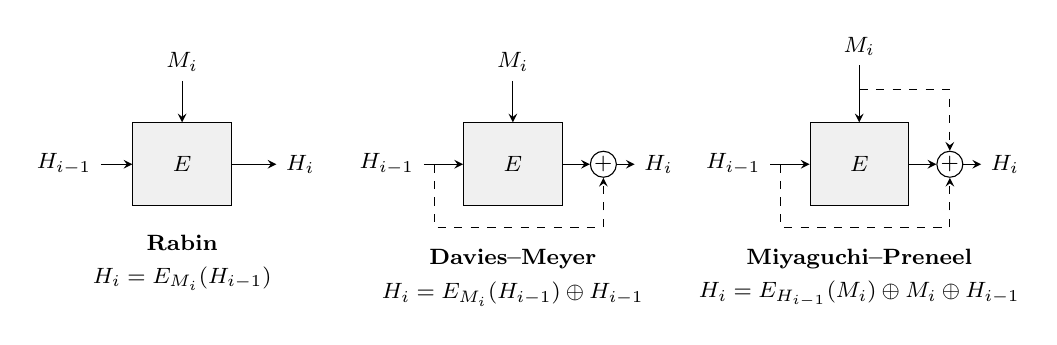
\begin{tikzpicture}[font=\footnotesize, >=stealth,
  enc/.style={draw, fill=gray!12, minimum width=1.25cm, minimum height=1.05cm, align=center},
  xo/.style={draw, circle, inner sep=0pt, minimum size=0.33cm}]
% Rabin
\node[enc] (e1) at (0,0) {$E$};
\node (m1) at (0,1.3) {$M_i$}; \node (h1) at (-1.5,0) {$H_{i-1}$}; \node (o1) at (1.5,0) {$H_i$};
\draw[->] (m1) -- (e1); \draw[->] (h1) -- (e1); \draw[->] (e1) -- (o1);
\node at (0,-1.0) {\textbf{Rabin}};
\node at (0,-1.45) {$H_i = E_{M_i}(H_{i-1})$};
% Davies-Meyer
\begin{scope}[xshift=4.2cm]
\node[enc] (e2) at (0,0) {$E$};
\node (m2) at (0,1.3) {$M_i$}; \node (h2) at (-1.6,0) {$H_{i-1}$};
\node[xo] (x2) at (1.15,0) {$+$}; \node (o2) at (1.85,0) {$H_i$};
\draw[->] (m2) -- (e2); \draw[->] (h2) -- (e2); \draw[->] (e2) -- (x2); \draw[->] (x2) -- (o2);
\draw[->, dashed] (-1.0,0) |- (0.6,-0.8) -| (x2);
\node at (0,-1.2) {\textbf{Davies--Meyer}};
\node at (0,-1.65) {$H_i = E_{M_i}(H_{i-1}) \oplus H_{i-1}$};
\end{scope}
% Miyaguchi-Preneel
\begin{scope}[xshift=8.6cm]
\node[enc] (e3) at (0,0) {$E$};
\node (m3) at (0,1.5) {$M_i$}; \node (h3) at (-1.6,0) {$H_{i-1}$};
\node[xo] (x3) at (1.15,0) {$+$}; \node (o3) at (1.85,0) {$H_i$};
\draw[->] (m3) -- (e3); \draw[->] (h3) -- (e3); \draw[->] (e3) -- (x3); \draw[->] (x3) -- (o3);
\draw[->, dashed] (-1.0,0) |- (0.6,-0.8) -| (x3);
\draw[->, dashed] (0,0.95) -| (x3);
\node at (0,-1.2) {\textbf{Miyaguchi--Preneel}};
\node at (0,-1.65) {$H_i = E_{H_{i-1}}(M_i) \oplus M_i \oplus H_{i-1}$};
\end{scope}
\end{tikzpicture}
\end{center}
In the Rabin and Davies--Meyer pictures the block $M_i$ enters as the \emph{key} (from above) and $H_{i-1}$ as the plaintext; in Miyaguchi--Preneel it is the other way round: $M_i$ is the plaintext and $H_{i-1}$ the key (slide 45). Dashed lines are the feed-forward XORs.

\textbf{Rabin scheme.} Rabin plugs a block cipher directly into Merkle--Damg\aa rd: the message block is used as the key, the previous digest as the plaintext, and the ciphertext is the new digest, $H_i = E_{M_i}(H_{i-1})$. The digest size equals the cipher's block size, so with DES the digest is only 64 bits. Although the scheme is very simple, it is subject to a \textbf{meet-in-the-middle attack}. Because Eve knows every key (the message blocks are her choice), each step can be run \emph{backwards}: $H_{i-1} = D_{M_i}(H_i)$. To forge a message with a given digest $H_t$, she encrypts forward from $H_0$ with about $2^{m/2}$ random choices of the first half of the blocks, stores the intermediate values, then decrypts backward from $H_t$ with about $2^{m/2}$ random choices of the second half, and looks for a common intermediate value. A match gives a full message with digest $H_t$ after only about $2 \times 2^{m/2}$ operations instead of $2^m$; for DES that is about $2^{32}$, which is feasible.

\textbf{Davies--Meyer scheme.} Davies--Meyer is the Rabin scheme plus a \textbf{feed-forward}: the previous digest is XORed onto the cipher output, $H_i = E_{M_i}(H_{i-1}) \oplus H_{i-1}$. Since $H_{i-1}$ now appears both inside the encryption and in the XOR, knowing $H_i$ and $M_i$ no longer lets Eve compute $H_{i-1}$ by decryption, so the backward half of the meet-in-the-middle attack is blocked. This is the protection the slide refers to.

\textbf{Matyas--Meyer--Oseas scheme} (Forouzan, not on the slides). This is the dual of Davies--Meyer: the previous digest is the key (passed through a function $g$ that adapts it to the key size) and the message block is the plaintext, with the block fed forward, $H_i = E_{g(H_{i-1})}(M_i) \oplus M_i$. It is useful when the key and block sizes of the cipher are equal.

\textbf{Miyaguchi--Preneel scheme.} To make the algorithm stronger, the plaintext, the cipher key and the ciphertext are all XORed together to create the new digest: $H_i = E_{H_{i-1}}(M_i) \oplus M_i \oplus H_{i-1}$. It is Matyas--Meyer--Oseas with the chaining value also fed forward. Whirlpool (below) is built on this scheme.

\subsection{SHA-512: overview and parameters \hot}
\asked{End-sem 2025--26 Q5 (7 marks): explain SHA-512 design: message preparation, word expansion, compression function, structure of each round.}
\likely{``Explain SHA-512 with a block diagram: padding, word expansion, round function'' (4--5 marks).}

SHA-512 is the member of the SHA-2 family with the longest digest. It follows the Merkle--Damg\aa rd scheme exactly: the message is padded and given a length field, split into 1024-bit blocks, and each block is fed with the previous 512-bit digest into a compression function; the output of the last block is the 512-bit digest.

\begin{center}
\begin{tikzpicture}[font=\footnotesize, >=stealth,
  blk/.style={draw, minimum width=2.0cm, minimum height=0.55cm},
  cf/.style={draw, fill=acc!8, minimum width=1.9cm, minimum height=0.8cm, align=center}]
\node[blk] (b1) at (0,1.6) {Block 1};
\node[blk] (b2) at (2.6,1.6) {Block 2};
\node (bd) at (4.1,1.6) {$\cdots$};
\node[blk] (bn) at (5.6,1.6) {Block $N$};
\draw[decorate,decoration={brace,amplitude=4pt}] ([yshift=2pt]b1.north west) -- node[above=4pt]{augmented message: a multiple of 1024-bit blocks} ([yshift=2pt]bn.north east);
\node[draw, align=center] (iv) at (-2.4,0) {Initial value\\512 bits};
\node[cf] (c1) at (0,0) {Compression\\function};
\node[cf] (c2) at (2.6,0) {Compression\\function};
\node (cd) at (4.1,0) {$\cdots$};
\node[cf] (cn) at (5.6,0) {Compression\\function};
\node[draw, fill=gold!20, align=center] (dg) at (7.9,0) {Digest\\512 bits};
\draw[->] (b1) -- (c1); \draw[->] (b2) -- (c2); \draw[->] (bn) -- (cn);
\draw[->] (iv) -- (c1); \draw[->] (c1) -- node[above]{512} (c2); \draw[->] (c2) -- (cd); \draw[->] (cd) -- (cn); \draw[->] (cn) -- (dg);
\end{tikzpicture}
\end{center}

SHA-512 is \textbf{word oriented}: a word is 64 bits. Each 1024-bit message block is 16 words, and the 512-bit digest is 8 words, named $A, B, C, D, E, F, G, H$. The parameters are: maximum message length $2^{128} - 1$ bits, block 1024 bits, digest 512 bits, 80 rounds per block, 64-bit words, 80 round constants $K_0, \dots, K_{79}$, and 80 expanded words $W_0, \dots, W_{79}$ per block.

\subsection{SHA-512: padding and length field \new}
\likely{``Compute the number of padding bits for a message of length $L$; is padding needed if the length is already a multiple of 1024?'' (2--3 marks).}

Before processing, Merkle--Damg\aa rd requires the message to be a whole number of blocks, with its length recorded at the end. SHA-512 therefore appends two things to the original message $M$: \textbf{padding}, which is a single 1 bit followed by as many 0 bits as needed, and a \textbf{128-bit length field} holding $|M|$ as an unsigned integer (this is why the maximum message length is $2^{128} - 1$). The total $|M| + |P| + 128$ must be a multiple of 1024, so
\[
|M| + |P| + 128 \equiv 0 \pmod{1024} \quad\Longrightarrow\quad \boxed{\,|P| = (-|M| - 128) \bmod 1024\,}, \qquad 0 \le |P| \le 1023 .
\]
Since the mod gives a value from 0 to 1023, the padding is always less than one block.

\begin{worked}[: padding (Forouzan Example 12.1)]
\textbf{Q.} What is the number of padding bits if the length of the original message is 2590 bits?

\textbf{A.} $|P| = (-2590 - 128) \bmod 1024 = (-2718) \bmod 1024$. Since $-2718 + 3 \times 1024 = 354$, $|P| = \mathbf{354}$ bits: a 1 followed by 353 zeros.\\
\emph{Check}: $2590 + 354 + 128 = 3072 = 3 \times 1024$, so the augmented message is exactly 3 blocks.
\end{worked}

\begin{worked}[: padding, new example]
\textbf{Q.} A message of 5000 bits is hashed with SHA-512. Find the number of padding bits, the number of blocks, and the content of the length field.

\textbf{A.} $|P| = (-5000 - 128) \bmod 1024 = (-5128) \bmod 1024 = -5128 + 6 \times 1024 = \mathbf{1016}$ bits (a 1 followed by 1015 zeros).\\
Total $= 5000 + 1016 + 128 = 6144 = \mathbf{6}$ \textbf{blocks}. The 128-bit length field holds $5000 = $ \ttx{1388} in hex, i.e.\ 115 zero bits followed by \ttx{1001110001000}.\\
\emph{Check}: $6144 / 1024 = 6$ exactly.
\end{worked}

\textbf{Edge cases (Forouzan Examples 12.2--12.3).} A message whose length is \emph{already} a multiple of 1024 still needs padding, because the length field must be added: for $|M| = 1024$, $|P| = (-1152) \bmod 1024 = 896$ and the result is 2 blocks. The formula gives the \textbf{minimum} padding $|P| = 0$ when $|M| \equiv 896 \pmod{1024}$ (the message plus the length field already fill the block) and the \textbf{maximum} $|P| = 1023$ when $|M| \equiv 897 \pmod{1024}$. In the actual standard (FIPS 180) the single 1 bit is always appended, so the padding is at least 1 bit; for $|M| \equiv 896$ this forces a full extra block of 1024 padding bits. A short check of the real rule: the 24-bit message ``abc'' gets $(-24 - 128) \bmod 1024 = 872$ padding bits and fits in one block.

\begin{trap}[: padding arithmetic]
Take the mod of a negative number correctly: add multiples of 1024 until the value lies in $0$--$1023$. Do not forget the 128-bit length field (SHA-1 and SHA-256 use a 64-bit field and 512-bit blocks, giving $|P| = (-|M| - 64) \bmod 512$).
\end{trap}

\subsection{SHA-512: word expansion and the compression function \new}

\textbf{Word expansion.} Each round uses one 64-bit word, but a block has only 16 words, so the block is expanded to 80 words $W_0, \dots, W_{79}$. The first 16 are the block itself; each later word mixes four earlier ones:
\[
W_i = W_{i-16} \oplus \mathrm{RotShift}_{1\text{-}8\text{-}7}(W_{i-15}) \oplus W_{i-7} \oplus \mathrm{RotShift}_{19\text{-}61\text{-}6}(W_{i-2}), \qquad 16 \le i \le 79,
\]
\[
\mathrm{RotShift}_{l\text{-}m\text{-}n}(x) = \mathrm{RotR}_l(x) \oplus \mathrm{RotR}_m(x) \oplus \mathrm{ShL}_n(x),
\]
where $\mathrm{RotR}_i(x)$ rotates $x$ right by $i$ bits (bits leaving on the right re-enter on the left) and $\mathrm{ShL}_i(x)$ shifts $x$ left by $i$ bits, filling with 0s (bits leaving are lost). This is the slides' (Forouzan's) form; see the correction box for the standard's exact operations. Since every later word depends on several earlier ones, a change in one message bit spreads into many of the 80 words.

\textbf{Initial values and constants.} The eight words of $H_0$ are the first 64 bits of the fractional parts of the square roots of the first eight primes (2 to 19); for example $A_0 = $ \ttx{6A09E667F3BCC908} from $\sqrt 2$. The 80 round constants $K_0, \dots, K_{79}$ are the first 64 bits of the fractional parts of the cube roots of the first 80 primes (2 to 409); for example $K_0 = $ \ttx{428A2F98D728AE22} from $\sqrt[3]{2}$. Taking them from irrational numbers shows that the designers hid no trapdoor in the constants (``nothing up my sleeve'' numbers).

\textbf{Compression function.} Processing one block takes 80 rounds. At the start, the eight digest words from the previous block (or the IV) are saved in eight temporary variables. Round $i$ mixes the current $A, \dots, H$ with the word $W_i$ and the constant $K_i$ and produces a new set of eight words. After round 79, the saved values are added to the outputs word by word modulo $2^{64}$; this \textbf{final adding} produces the digest that is passed to the next block (or is the final digest). The final adding is a feed-forward, exactly like Davies--Meyer, and it makes the compression function impossible to run backwards.

\textbf{Structure of each round.} Six of the eight words are simply moved one place right, and only two new words are computed, using two mixers (every $+$ here is addition modulo $2^{64}$):
\[
T_1 = H + \mathrm{Conditional}(E, F, G) + \mathrm{Rotate}(E) + W_i + K_i, \qquad T_2 = \mathrm{Majority}(A, B, C) + \mathrm{Rotate}(A),
\]
\[
H \leftarrow G,\; G \leftarrow F,\; F \leftarrow E,\; E \leftarrow D + T_1,\; D \leftarrow C,\; C \leftarrow B,\; B \leftarrow A,\; A \leftarrow T_1 + T_2 .
\]
The three functions are bitwise (except Rotate, which moves bits within the word):
\begin{itemize}[nosep]
  \item $\mathrm{Majority}(x, y, z) = (x \wedge y) \oplus (y \wedge z) \oplus (z \wedge x)$: each output bit is the majority value of the three input bits.
  \item $\mathrm{Conditional}(x, y, z) = (x \wedge y) \oplus (\overline{x} \wedge z)$: each bit of $x$ acts as a selector, taking the bit of $y$ where $x = 1$ and the bit of $z$ where $x = 0$ (``if $x$ then $y$ else $z$'').
  \item $\mathrm{Rotate}(x) = \mathrm{RotR}_{28}(x) \oplus \mathrm{RotR}_{34}(x) \oplus \mathrm{RotR}_{39}(x)$.
\end{itemize}

\begin{center}
\begin{tikzpicture}[font=\footnotesize, >=stealth,
  reg/.style={draw, fill=gray!15, minimum width=0.85cm, minimum height=0.45cm, inner sep=1pt},
  mix/.style={draw, fill=acc!8, align=center, inner sep=3pt}]
\foreach \n [count=\i] in {A,B,C,D,E,F,G,H} {
  \node[reg] (t\n) at (\i*1.0,3.2) {\n};
  \node[reg] (b\n) at (\i*1.0,0) {\n};
}
\foreach \a/\b in {A/B,B/C,C/D,E/F,F/G,G/H} \draw[->] (t\a.south) -- (b\b.north);
\node[mix] (m2) at (10.6,1.9) {Mixer 2: $T_1 = H + \mathrm{Cond}(E,F,G)$\\$+ \mathrm{Rotate}(E) + W_i + K_i$};
\node[mix] (m1) at (10.6,0.8) {Mixer 1: $T_2 = \mathrm{Maj}(A,B,C)$\\$+ \mathrm{Rotate}(A)$};
\node[font=\footnotesize, fill=white, inner sep=1pt] (xa) at (1.0,1.6) {$T_1 + T_2$};
\node[font=\footnotesize, fill=white, inner sep=1pt] (xe) at (5.0,1.6) {$D + T_1$};
\draw[->] (xa) -- (bA.north); \draw[->] (xe) -- (bE.north);
\node[left=2pt of tA] {in:};
\node[left=2pt of bA] {out:};
\end{tikzpicture}
\end{center}
In Forouzan's notation the new $A$ is called $X$ and the new $E$ is $Y$. Because $A$ and $E$ change every round and the other six words are shifted, every input word affects all eight words within a few rounds.

\begin{mustknow}[: SHA-512 in numbers]
Block 1024 bits $=$ 16 words of 64 bits; digest 512 bits $=$ 8 words $A$--$H$; 80 rounds; 80 words $W_0$--$W_{79}$; 80 constants $K_i$; length field 128 bits; $|P| = (-|M| - 128) \bmod 1024$; max message $2^{128} - 1$ bits; final adding modulo $2^{64}$.
\end{mustknow}

\subsection{Exercises on the SHA-512 operations \new}
\likely{One of the slide exercises (RotR, ShL, Conditional, Majority, Rotate) on given hex words.}

The slide exercises use a \textbf{128-bit} $x$ (real SHA-512 words are 64 bits) and work in hex: a rotation or shift by 12 bits moves the string by 3 hex digits. All results below were recomputed.
\[
x = \texttt{1234 5678 ABCD 2345 3456 5678 ABCD 2468}
\]

\begin{worked}[: RotR, ShL, Conditional, Majority, Rotate (slides 52--56)]
\textbf{RotR$_{12}(x)$.} Rotate right by 12 bits $=$ 3 hex digits: the last three digits \ttx{468} move to the front.\\
\ttx{4681 2345 678A BCD2 3453 4565 678A BCD2}

\textbf{ShL$_{12}(x)$.} Shift left by 3 hex digits: the first three digits \ttx{123} are lost and three 0 digits enter on the right.\\
\ttx{4567 8ABC D234 5345 6567 8ABC D246 8000}

\textbf{Conditional$(x, y, z)$} with $y = $ \ttx{2234 5678 \dots}, $z = $ \ttx{3234 5678 \dots} (the three words differ only in the first digit). For the first digit, $x = 0001$ selects $y$ where $x = 1$ and $z$ where $x = 0$: $(0001 \wedge 0010) \oplus (1110 \wedge 0011) = 0000 \oplus 0010 = 0010 = 2$. For every other digit the three inputs are equal, and Conditional of three equal digits is that digit.\\
Result: \ttx{2234 5678 ABCD 2345 3456 5678 ABCD 2468}

\textbf{Majority$(x, y, z)$}, same $x, y, z$. First digit: $(0001 \wedge 0010) \oplus (0010 \wedge 0011) \oplus (0011 \wedge 0001) = 0000 \oplus 0010 \oplus 0001 = 0011 = 3$. The other digits are unchanged.\\
Result: \ttx{3234 5678 ABCD 2345 3456 5678 ABCD 2468}

\textbf{Rotate$(x) = \mathrm{RotR}_{28}(x) \oplus \mathrm{RotR}_{34}(x) \oplus \mathrm{RotR}_{39}(x)$.} First the three rotations, then the XOR:\\[2pt]
{\small
\begin{tabular}{@{}ll@{}}
$\mathrm{RotR}_{28}(x)$ & \ttx{BCD2 4681 2345 678A BCD2 3453 4565 678A}\\
$\mathrm{RotR}_{34}(x)$ & \ttx{2AF3 491A 048D 159E 2AF3 48D1 4D15 959E}\\
$\mathrm{RotR}_{39}(x)$ & \ttx{F157 9A48 D024 68AC F157 9A46 8A68 ACAC}\\
\midrule
Rotate$(x)$ & \ttx{6776 95D3 F7EC 1AB8 6776 E6C4 8218 5EB8}
\end{tabular}}\\[2pt]
$\mathrm{RotR}_{28}$ is a rotation by 7 hex digits, so it can be done digit-wise; $\mathrm{RotR}_{34}$ and $\mathrm{RotR}_{39}$ are not multiples of 4 and must be done in binary.
\end{worked}

\begin{worked}[: new exercise on 16-bit and 64-bit words]
\textbf{Q.} (a) For the 16-bit words $x = $ \ttx{F0F0}, $y = $ \ttx{AAAA}, $z = $ \ttx{5555}, find Conditional$(x, y, z)$ and Majority$(x, y, z)$. (b) For the 64-bit word $w = $ \ttx{0123 4567 89AB CDEF}, find $\mathrm{RotR}_8(w)$ and $\mathrm{ShL}_8(w)$.

\textbf{A.} (a) Conditional takes $y$ where $x$ is 1 and $z$ where $x$ is 0. $x \wedge y = $ \ttx{A0A0}, $\overline x \wedge z = $ \ttx{0F0F} $\wedge$ \ttx{5555} $= $ \ttx{0505}; Conditional $= $ \ttx{A0A0} $\oplus$ \ttx{0505} $= \mathbf{A5A5}$.\\
Majority: $x \wedge y = $ \ttx{A0A0}, $y \wedge z = $ \ttx{0000} (since $z = \overline y$), $z \wedge x = $ \ttx{5050}; XOR $= \mathbf{F0F0}$. This equals $x$, as it must: $y$ and $z$ disagree in every bit, so $x$ always casts the deciding vote.\\
(b) 8 bits $=$ 2 hex digits. $\mathrm{RotR}_8(w) = $ \ttx{EF01 2345 6789 ABCD} (\ttx{EF} wraps to the front); $\mathrm{ShL}_8(w) = $ \ttx{2345 6789 ABCD EF00} (\ttx{01} is lost, \ttx{00} enters).
\end{worked}

\subsection{Whirlpool}
Whirlpool, designed by Rijmen and Barreto and selected by the NESSIE project (New European Schemes for Signatures, Integrity, and Encryption), is an iterated hash function based on the \textbf{Miyaguchi--Preneel} scheme, in which the compression function is a block cipher: $H_i = E_{H_{i-1}}(M_i) \oplus M_i \oplus H_{i-1}$. The cipher, called W, is a \textbf{modified AES} tailored for this purpose.

\textbf{Parameters.} Block size 512 bits, digest 512 bits, cipher key 512 bits (the previous digest), initial value $H_0$ all 0s, and maximum message length $2^{256} - 1$ bits. The message is padded (a 1 followed by 0s) to an \emph{odd} multiple of 256 bits and then a \textbf{256-bit length field} is appended; an odd multiple of 256 plus 256 is an even multiple, i.e.\ a multiple of 512. For example, $|M| = 1000$ needs $|P| = (-1000 - 256) \bmod 512 = 280$ padding bits, since $1000 + 280 = 1280 = 5 \times 256$ (odd) and $1280 + 256 = 1536 = 3 \times 512$.

\textbf{How the Whirlpool cipher differs from AES.} It uses the same four kinds of transformation, but on a larger state and with all rounds alike:
\begin{itemize}[nosep]
  \item The block and key are 512 bits, held as an $8 \times 8$ matrix of bytes (AES: 128 bits as $4 \times 4$).
  \item There are 10 rounds, each with SubBytes, \textbf{ShiftColumns} (column $j$ is rotated down by $j$ positions, instead of AES's ShiftRows), \textbf{MixRows} (each row is multiplied by a fixed $8 \times 8$ circulant matrix, instead of AES's MixColumns) and AddRoundKey.
  \item Arithmetic is in GF$(2^8)$ with modulus $x^8 + x^4 + x^3 + x^2 + 1$ (AES uses $x^8 + x^4 + x^3 + x + 1$), and the S-box is built from smaller 4-bit boxes.
  \item The round keys are generated by running the same round function on the key, with round constants taken from the S-box in place of a key, instead of AES's separate key-expansion routine.
\end{itemize}

\begin{fixbox}
\begin{itemize}[nosep]
  \item Slide 27: ``$0.69 \times 2^{34}$ seconds or more than 500 years''. In fact $0.69 \times 2^{34}$ s $\approx 376$ years ($2^{34}$ s alone is $\approx 544$ years). The conclusion (secure against preimage attacks) stands.
  \item Slides 54--55 swap the binary for the first digit: Conditional$(0001, 0010, 0011) = 0010 = 2$ and Majority$(0001, 0010, 0011) = 0011 = 3$; the slides print 0011 for Conditional and 0010 for Majority, though the hex results 2 and 3 are right. Both slides also label the third word $x$ instead of $z$.
  \item The exercise $x$ (slides 52--56) is 128 bits, though real SHA-512 words are 64 bits; the rotations on the slides are done on 128 bits, and the results above follow the slides.
  \item Slide 11 prints Problem 4 as $P \approx 1 - e^{-k^2/2N}$; that formula would give $k = 1.18\sqrt N$. The correct one is $P \approx 1 - e^{-k^2/N}$ (as on slide 35), which gives $k = 0.83\sqrt N = 16$.
  \item Slide 40 lists SHA under the ``block cipher'' approach. Forouzan classifies MD and SHA as compression functions \emph{made from scratch} and Rabin, Davies--Meyer, Matyas--Meyer--Oseas and Miyaguchi--Preneel as block-cipher based; write it that way in the exam.
  \item Slides 48 and 51 (from Forouzan) simplify the standard: in FIPS 180 the word expansion uses addition modulo $2^{64}$ and a \emph{right} shift (SHR), not XOR and ShL, and Rotate$(E)$ uses $\mathrm{RotR}_{14} \oplus \mathrm{RotR}_{18} \oplus \mathrm{RotR}_{41}$, not 28-34-39. The slide's ``ShL\dots padding the left by 0s'' is self-contradictory (a left shift fills on the right). For the exam, use the slide formulas.
\end{itemize}
\end{fixbox}
